\documentclass[12pt]{article}

\usepackage{fontawesome}
\usepackage{hyperref}
\usepackage{xurl}
\usepackage{graphicx}
\usepackage{float}
\usepackage[tagged, highstructure]{accessibility}
\usepackage{bookmark}
\usepackage{enumitem}

\hypersetup{
    colorlinks=false,
    pdfborder={0 0 0},
    pdftitle={Networking and Firewalls},
    pdfauthor={Adrianna Holden-Gouveia},
    pdfsubject={Information Security - Lab Assignment},
    pdflang={en-US},
    pdfkeywords={firewalls, ports, ShieldsUP, network security}
}

% Configure PDF bookmarks for navigation
\bookmarksetup{
    numbered,
    open,
}

% Configure list spacing for better accessibility
\setlist{nosep}



\title{Networking and Firewalls}
\author{
        Adrianna Holden-Gouveia \\
        Website: \href{https://aholdengouveia.name}{aholdengouveia.name}\\ 
        \date{\vspace{-5ex}}
        %Email: \href{mailto:admin@aholdengouveia.name}{admin@aholdengouveia.name} \\
%        \faLinkedin{: aholdengouveia} \\
        \faGithub {: aholdengouveia} \\
        \faTwitter {: aholdengouveia} \\
        }

%S\date{\today}


\begin{document}    

\maketitle

\section*{Accessibility Notice}
This document is also available in HTML format at:

Link: \href{https://aholdengouveia.name/InfoSec/labs/firewalls.html}{\textbf{\nolinkurl{https://aholdengouveia.name/InfoSec/labs/firewalls.html}}}

The HTML version provides enhanced accessibility features including keyboard navigation, screen reader support, responsive design, dark mode support, and high contrast options.


%\begin{abstract}
%This is a template for Linux Administration Lab work
%\end{abstract}
%\tableofcontents

\section*{Learning Outcomes}
By the end of this lab, you will be able to:
\begin{itemize}
    \item Explain what a firewall does, and how allow and deny rules work
    \item Compare how two different networks look from the internet
    \item Create and test firewall rules for a scenario
    \item Explain how rule order and the default policy change what a firewall allows
\end{itemize}

\section*{Lab Instructions}
Everything in this lab runs in your web browser, so you don't need to install anything. Both tools are linked under Resources.

\subsection*{Screenshots}
This lab asks for 6 screenshots. Each screenshot should have your name, term, and year.  One of the easiest ways to do that is make a text document with your name and term/year on your computer and save it to use all term. Any screenshots that don't include this information won't be counted.

\begin{figure}[H]
    \centerline{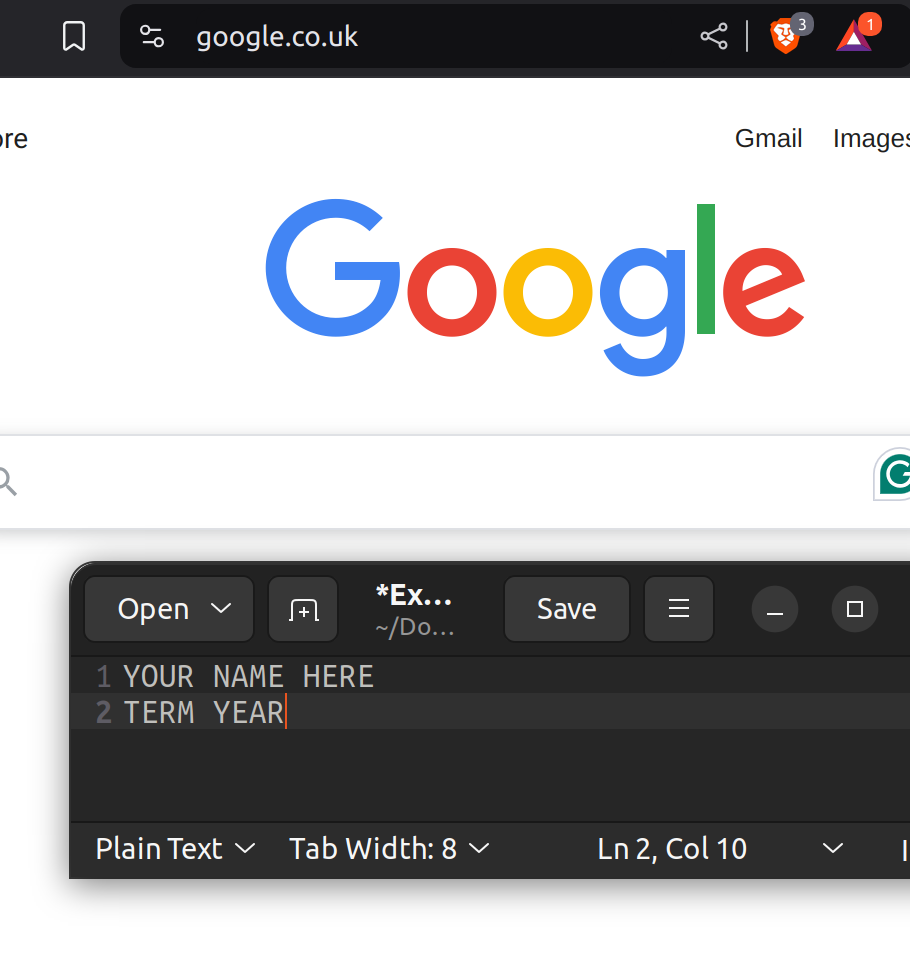
\includegraphics[scale=.2]{ExampleScreenshot.png}}
    \caption{This is an image of what each of your screenshots should look like}
    \alt{Example screenshot: a web browser showing the Google home page, with a small text editor window in front of it that says YOUR NAME HERE and TERM YEAR}
\end{figure}

\subsection*{Part 1: Your Network from the Outside}
ShieldsUP! is a free tool from Gibson Research Corporation. It checks your internet connection from the outside, the way an attacker would see it, and shows which common ports are open. This is a port scan, the same kind of scan attackers use during network reconnaissance to find a way in. It only checks the connection you're using, so you're only testing your own network.

Run it from \textbf{two different places}, such as home and school, or home and your phone's hotspot. Only use networks you're allowed to use. If your school doesn't allow this kind of test on its network, use home and your phone's hotspot instead.

At each place:
\begin{enumerate}
    \item Go to ShieldsUP!, select Proceed, then select Common Ports.
    \item Take a screenshot of the results. Each port is shown as Open, Closed, or Stealth.
    \item Write down where you were, such as home Wi-Fi or a phone hotspot, the date, and how many ports were Open, Closed, and Stealth.
\end{enumerate}
Then compare the two places:
\begin{enumerate}[start=4]
    \item What was different between the two results? What was the same?
    \item Why do you think they were different? Think about who runs each network, and what firewall or router is protecting it.
    \item Which network looks safer from the outside, and why?
    \item If any port was Open, what service uses that port? Does it need to be open?
\end{enumerate}

\subsection*{Part 2: Build Firewall Rules}
Open my Firewall Simulator. You're setting up the firewall for a small office's web server. The office network is 192.168.1.0/24. The server needs to:
\begin{itemize}
    \item Let anyone visit the website, using HTTP (port 80) and HTTPS (port 443)
    \item Let only the office use SSH (port 22) to manage the server
    \item Block everything else
\end{itemize}
\begin{enumerate}[start=8]
    \item Choose a default policy, and add rules to meet these needs.
    \item Select Test all traffic, and take a screenshot of your rules and the results.
    \item Explain each of your rules in a sentence, and why you chose your default policy.
    \item Add one piece of test traffic of your own, and explain what happened to it and why.
\end{enumerate}

\subsection*{Part 3: Rule Order and the Default Policy}
\begin{enumerate}[start=12]
    \item Select Load the rule order example, then Test all traffic. Take a screenshot. The office admin can't log in with SSH. Explain why, using what the simulator says.
    \item Fix it by changing the order of the rules, test again, and take a screenshot. Explain what you changed and why it worked.
    \item Change the default policy to allow all, and test again. What traffic gets through now that shouldn't? A deny all default works like an allowlist, and allow all works like a denylist. Why is deny all usually the safer default?
\end{enumerate}

\subsection*{Part 4: What Firewalls Can't Do}
\begin{enumerate}[start=15]
    \item A firewall allowed the web traffic in Part 2. Give one way an attacker could still cause harm through allowed traffic.
    \item Give one threat a firewall can't protect against, such as phishing, and explain why.
\end{enumerate}

\section*{Deliverables}
One file that includes:
\begin{itemize}
    \item Part 1: your 2 ShieldsUP! screenshots, where and when you ran each one, and your answers to the comparison questions
    \item Part 2: your screenshot of your rules and results, and your explanations
    \item Part 3: your 2 screenshots, and your explanations
    \item Part 4: your answers
\end{itemize}

\section*{Resources}
References, a video, a PowerPoint and some notes are available at my website
Link: \href{https://www.aholdengouveia.name/InfoSec/NetworkSecurity.html}{\textbf{\nolinkurl{https://www.aholdengouveia.name/InfoSec/NetworkSecurity.html}}}

ShieldsUP! from Gibson Research Corporation, for Part 1
Link: \href{https://www.grc.com/shieldsup}{\textbf{\nolinkurl{https://www.grc.com/shieldsup}}}

My Firewall Simulator, for Parts 2 and 3
Link: \href{https://www.aholdengouveia.name/InfoSec/labs/firewall-simulator.html}{\textbf{\nolinkurl{https://www.aholdengouveia.name/InfoSec/labs/firewall-simulator.html}}}

Common port numbers and the services that use them
Link: \href{https://en.wikipedia.org/wiki/List_of_TCP_and_UDP_port_numbers}{\textbf{\nolinkurl{https://en.wikipedia.org/wiki/List_of_TCP_and_UDP_port_numbers}}}

\end{document}